\subsection{USB Interface}
A USB Interface was included to serve two purposes:
\begin{itemize}
    \item Primary source of power to the system, supplying up to \SI{500}{mA} of current to charge the ultra-capacitors.
    \item Communication with the host machine; providing serial output for firmware debugging as well as controller configuration.
\end{itemize}

This was quickly extended to be the main port of control, as the device was to be powered via the USB port of a computer, also being able to configure the device (i.e set reference point) over USB was the natural next step. Doing so avoid the need to a design a hardware interface for controlling the device, which would have required a display and other peripherals. It was also likely that that control algorithms would be costly and therefore leave very little computation time for displaying graphics on an LCD display incorportated into the device.
%%%%%%%%%%%%%%%%%%%%%%%%%%%%%%%%%%%%%%%%%%%%%%%%%%%%%%%%%%%%%%%%%%%%%%%%%%%%%%%%

\subsubsection{USB to serial}
The FTDI FT232R USB to serial UART interface implements the USB protocol on a single chip, offloading the processing from the main microcontroller. This chip incorporates the high speed termination resistors and clock to further simplify the design \cite{ft232r}.
\begin{figure}
    \centering
    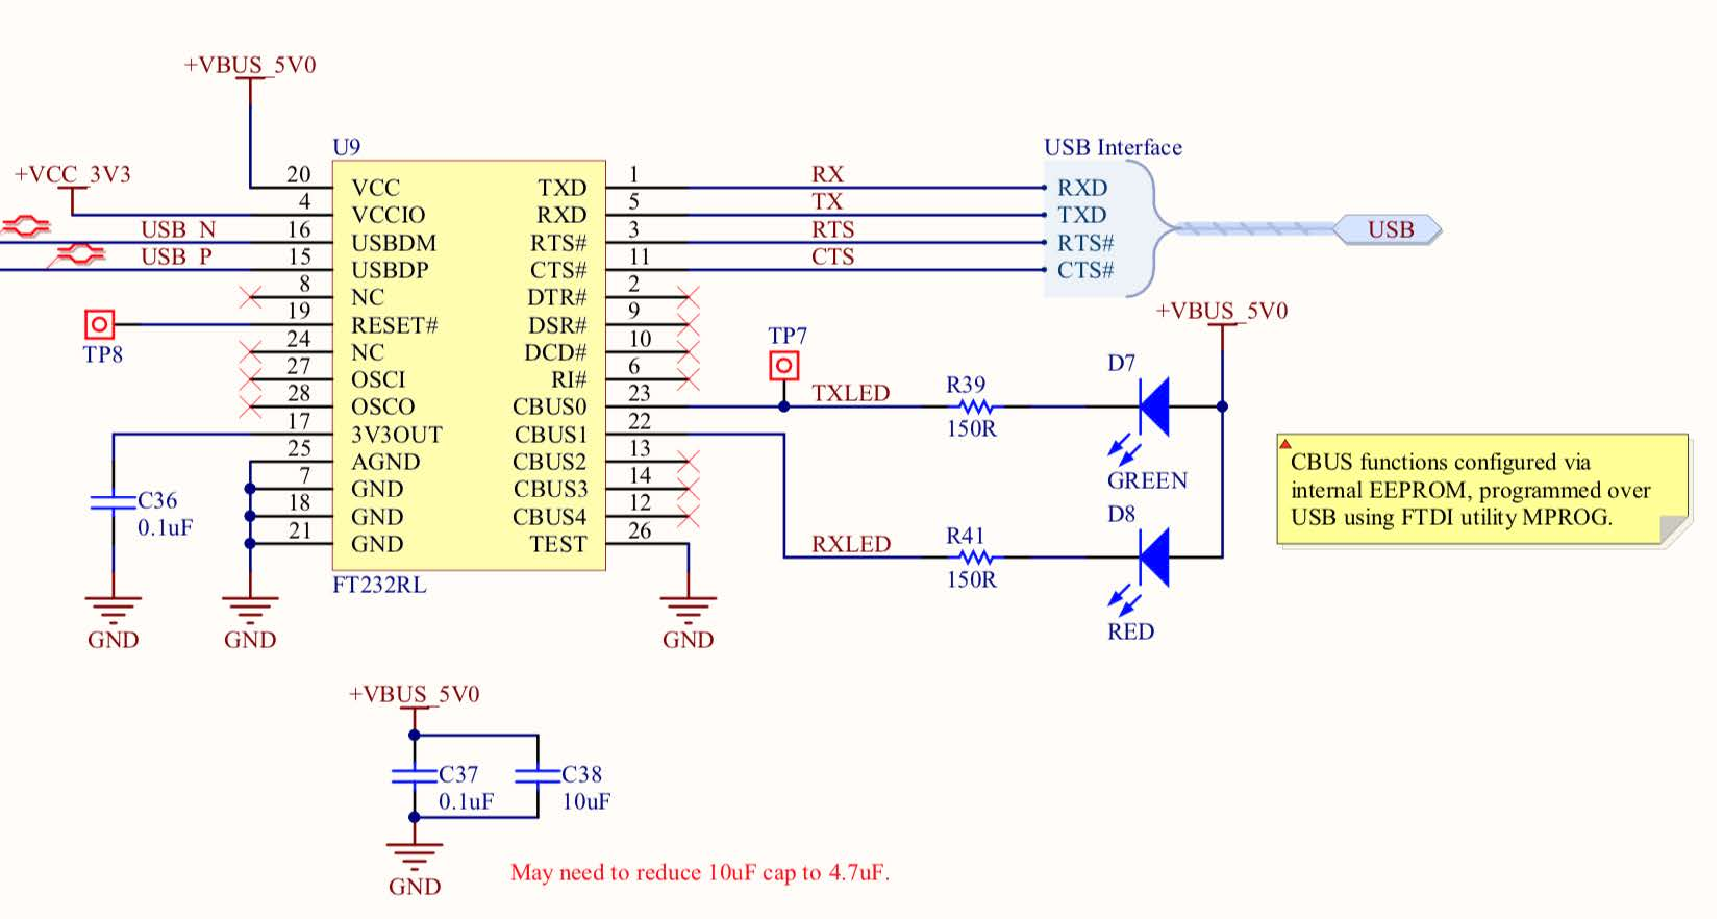
\includegraphics[height = 8cm]{figures/hardware/usb_schematic.pdf}
    \caption{USB schematic excerpt.}
    \label{fig:usb_schematic}
\end{figure}
To communicate with the MCU via UART requires two physical connections: one to receive data (RX) and one to transmit data (TX). These are connected to the opposite pins on each device. In the first prototype additional hand-shaking connections were included (RTS and CTS) in case they were required. Since each device were operating at similar rates to each other, that is they processes the data received via UART at similar rates, they did not require hand-shaking to add artificial wait time in between transmissions so one of the devices could wait for the other before transmitting the next byte. This ensure that data is not lost during the transmission process. 
\\ \\
Status LEDs were connected via current limiting resistors to the CBUS0 and CBUS1 pins of the FT232R. This allowed for visual feedback to confirm when data was being received and transmitted to the chip over UART, allowing for a simple check rather than having to connect and configure an oscilloscope or logic analyser each time.
\begin{itemize}
    \item The CBUS pins can be configured for a number of functions, one option sets the pins to be used as LED drivers for received/transmitted data. This is conveniently the default configuration of the device, which avoided having to externally program the EEPROM using software utility provided by the manufacturer (FTDI).
    \item Feature proved useful during debugging on a number of occasions.
\end{itemize}

It was important to ensure that \texttt{VCCIO} was connected to the same supply as the MCU, in this case \SI{3.3}{V}. In in the initial prototype this was connected to the MCU \SI{3.3}{V} voltage rail, which lead to some minor issues detailed below. In the final revision this pin was connected directly to the \texttt{3V3OUT} pin and hence uses the internal LDO regulator to supply the reference, this is the option recommended in the datasheet \cite{ft232r} and also improved the layout of the PCB (separated power rails, reduced noise that would couple off the line).

%%%%%%%%%%%%%%%%%%%%%%%%%%%%%%%%%%%%%%%%%%%%%%%%%%%%%%%%%%%%%%%%%%%%%%%%%%%%%%%%

\subsubsection{Power filtering and input protection}
Following the USB Hardware Design Guidelines \cite{usb_design_guide} recommends that a \SI{10}{nF} capacitor and a ferrite bead should be placed as close to the USB connector as possible. The ferrite bead in conduction with the capacitors in a PI configuration form an LC filter that helps to smooth the USB power supply \cite{usb_filtering}.
\begin{figure}
    \centering
    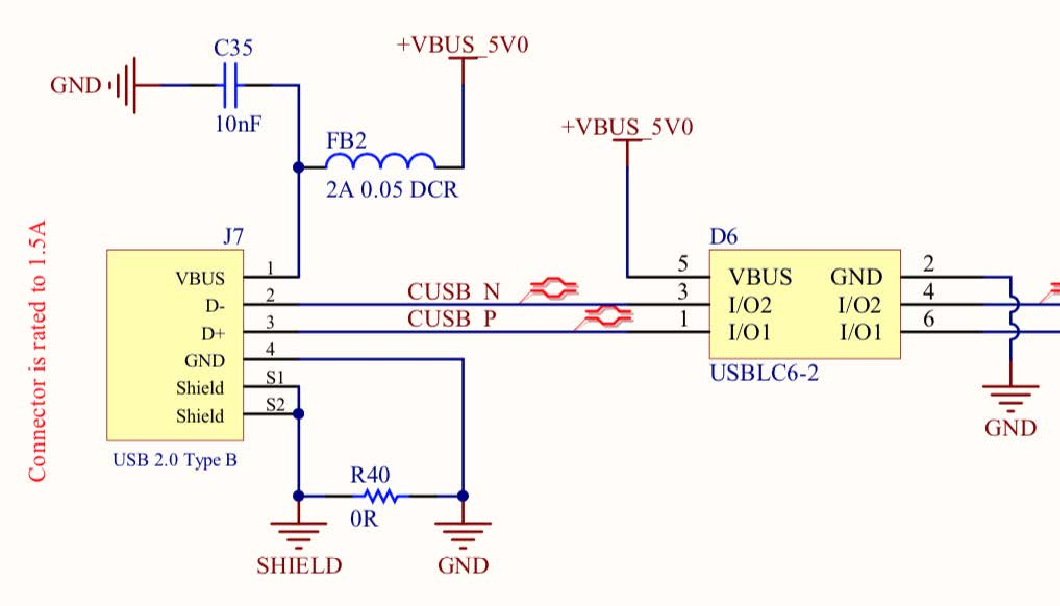
\includegraphics[height = 8cm]{figures/hardware/usb_power.pdf}
    \caption{USB power filtering and protection schematic excerpt.}
    \label{fig:usb_power}
\end{figure}
As shown in figure \ref{fig:usb_power}, a zero-ohm resistor was included between the shield and ground as the shield of a USB cable acts as an antenna. As such connecting the shield directly to the signal ground on the PCB should be avoided. In the case that EMI becomes and issues the zero-ohm resistor could be replaced with an inductor/ferrite bead.
\\ \\
Transient-voltage-suppressot (TVS) diodes are place as the first device next to the external USB connector to provide the shortest current path to ground in the case of an electrostatic discharge event were to occur. This minimises the possibility of damage elsewhere on the PCB.
%%%%%%%%%%%%%%%%%%%%%%%%%%%%%%%%%%%%%%%%%%%%%%%%%%%%%%%%%%%%%%%%%%%%%%%%%%%%%%%%